\documentclass{article}
\usepackage{hyperref}
\usepackage{graphicx}

\begin{document}

\section*{Hi, I'm Tony}
\begin{figure}[h]
    \centering
    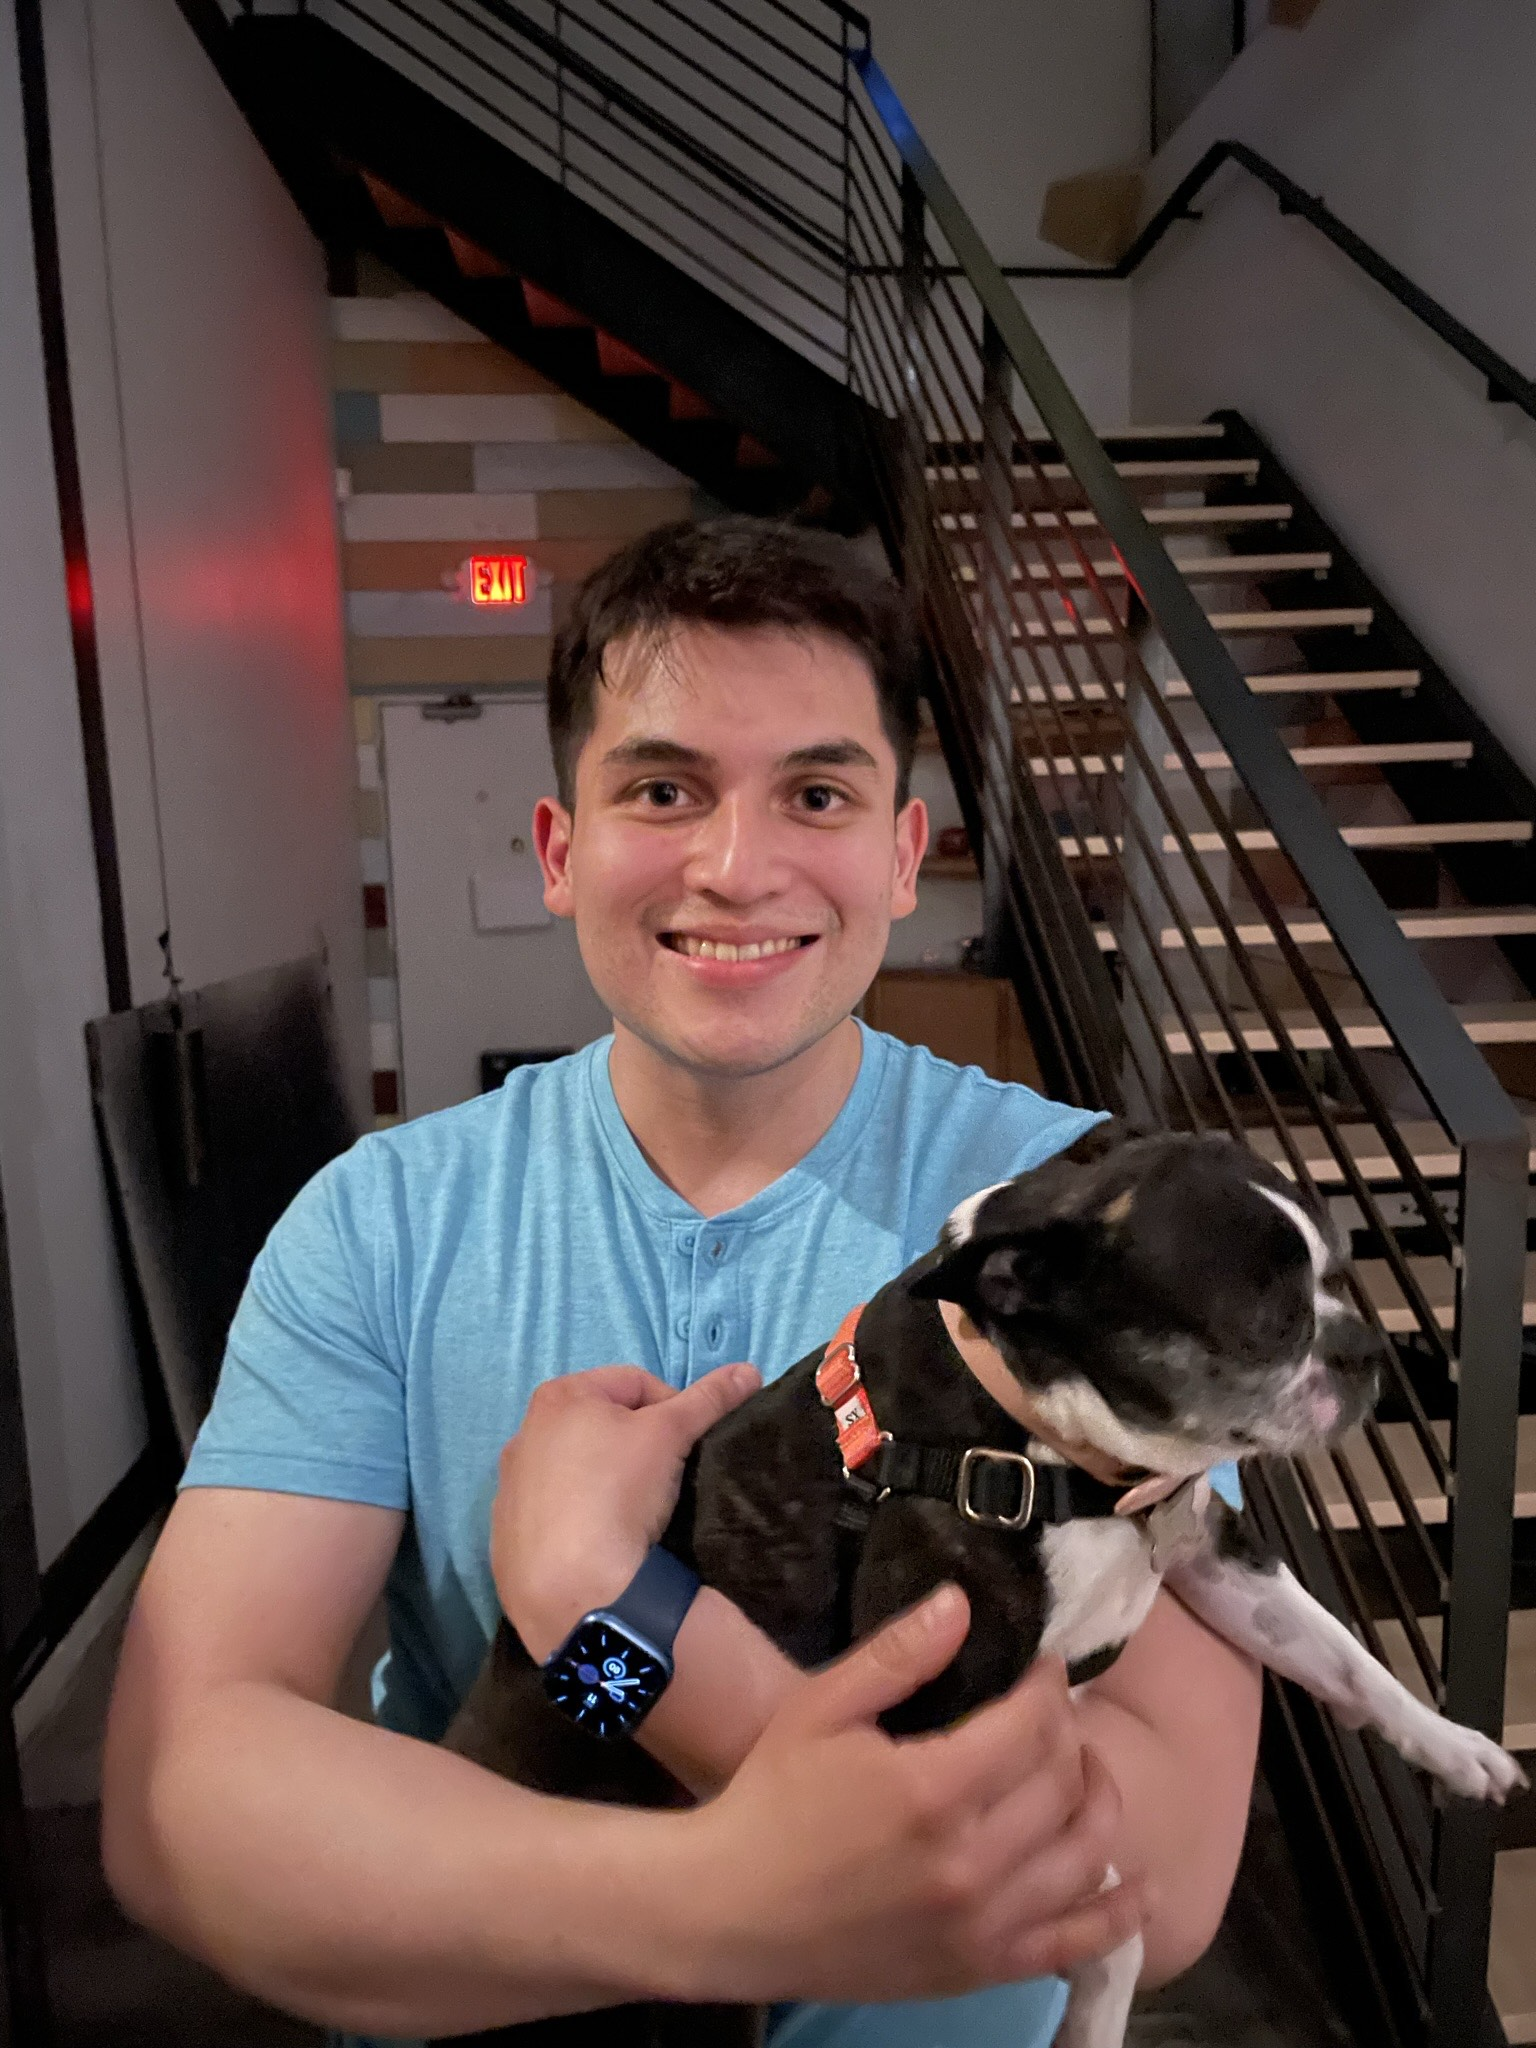
\includegraphics[width=0.3\textwidth]{static/images/myself.png}
    \caption{Tony Arriaza}
\end{figure}

\subsection*{ My background}

Hello, I'm Tony Arriaza. I'm 28 years old with experience primarily as a software engineer moving into the field of Machine Learning. In university I double majored in Mathematics and Computer Science. In undergraduate I focused on courses that would aid in Machine Learning. Such as Probability Theory,Mathematical Statistics, Deep Learning, Natural Language Processing, Artificial Intelligence, and Data Cleaning. After a few years of working as a Software Engineer I decided to pursue my passions related to Machine Learning and Artificial Intelligence. This website also has a few entries that I've written implementing Neural Networks from scratch, while also exploring the underlying Mathematics that allow these networks to function. 

\subsection*{Machine Learning From Scratch}

Here I have my exploration of Machine Learning from the ground up, using only numpy. I've written these for myself as a reference as well as a learning tool, after discovering that many online sources and even LLMs do a poor job at showing and describing the mathematics of these algorithms. Many sources will simply explain things at a high level because any library that can be used has an autograd system, that is a system that does most things anyone might need. However in many cases understanding *how* these autograd systems work is necessary to solve complex problems that may be outside of a basic domain. Furthermore, it is not always possible to rely on autograd systems, especially as Machine Learning becomes more important in areas where only low level languages are available, such as the defense industry. The goal of these notebooks is to outline a step by step approach on how one might develop a machine learning algorithm without access to an autograd system. Below is a list of Notebooks in the order I've written them

\begin{itemize}
    \item \textbf{Matrix Multiplication}: The very basics, Matrix Multiplication and its implementation.
    \begin{itemize}
        \item \href{/notebooks/StartingFromTheBasicsMatrixMultiplication.ipynb}{Matrix Multiplication}
    \end{itemize}
        \item \textbf{Linear Regression}: Explaining and implementing the underlying math of linear regression, and Gradient Descent
    \begin{itemize}
        \item \href{/notebooks/StartingFromTheBasicsLinearRegression.ipynb}{Linear Regression}
    \end{itemize}
    \item \textbf{Backpropagation}: Explaining and implementing the underlying math of Backpropagation in a basic Neural Network.
    \begin{itemize}
        \item \href{/notebooks/StartingFromTheBasicsBackPropagation.ipynb}{Back Propagation}
    \end{itemize}
    \item \textbf{Binary Classification}: Explaining Binary Classifcation and BackPropagation with Binary problems
    \begin{itemize}
        \item \href{/notebooks/StartingFromTheBasicsBinaryClassification.ipynb}{Binary Classification}
    \end{itemize}
    \item \textbf{Binary Classification}: Explaining Multi Class Classifcation and BackPropagation
    \begin{itemize}
        \item \href{StartingFromTheBasicsMultiClassClassification.ipynb}{Multi Class Classification}
    \end{itemize}
\end{itemize}




\end{document}
